\section{Activity Structure}

\todo{REFACTOR GIRAF COMPONENTS!}

\begin{figure}[h!]
	\centering
	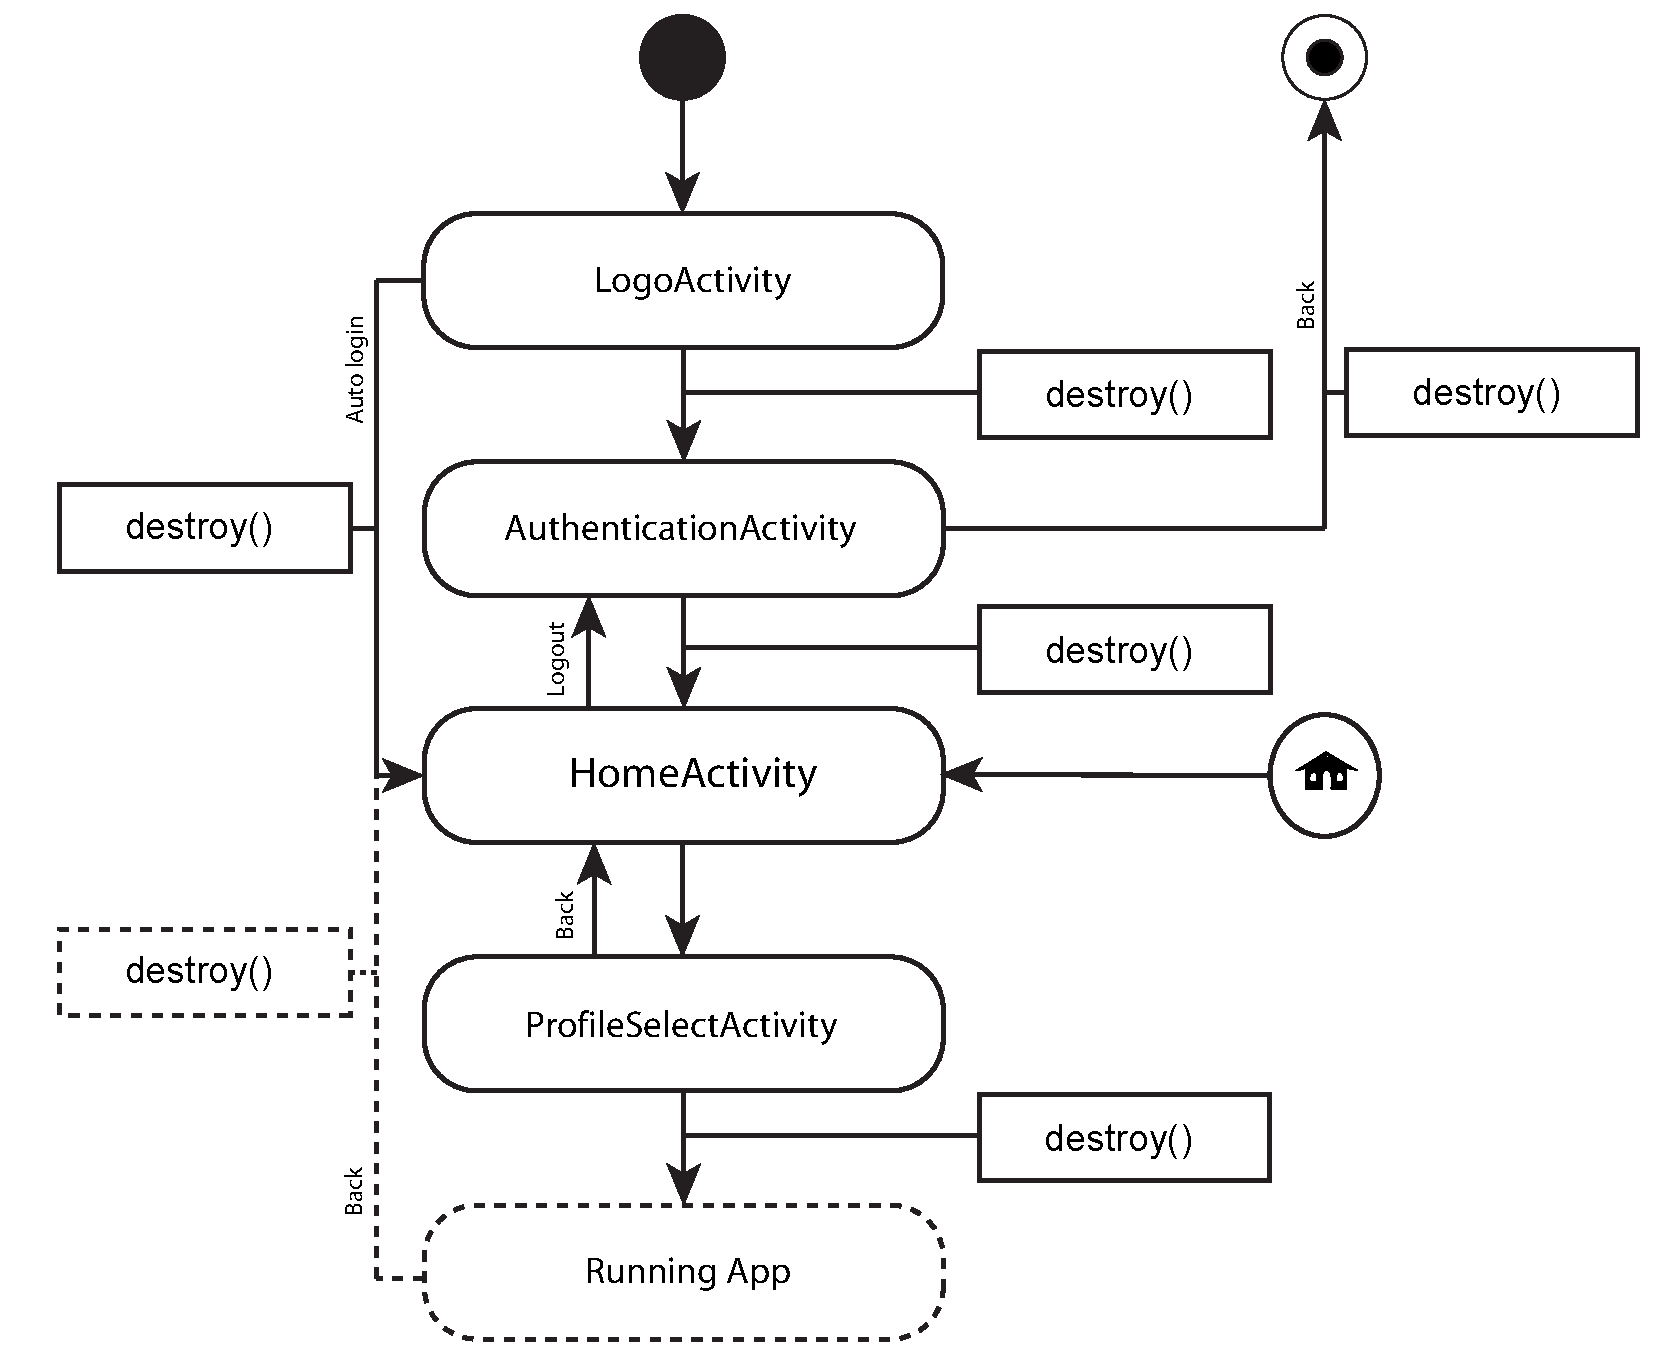
\includegraphics[width=1\textwidth]{gfx/activityDiagram.pdf}
	\caption{Activity diagram of the launcher}
	\label{fig:activity_diagram}
\end{figure}

Figure~\ref{fig:activity_diagram} shows the activity structure of the \giraf[] launcher. Every transition with a \verb+destroy()+ box on it gets the activity starting the transition destroyed. Everytime the user is outside the launcher and hits the home button they will end up in the \activity{HomeActivity}, if the \giraf[] launcher is set to the default launcher.